\documentclass[10pt,a4paper]{article}
\usepackage[margin=18mm]{geometry}
\usepackage[T1]{fontenc}
\DeclareUnicodeCharacter{0130}{I}
\DeclareUnicodeCharacter{0307}{}
\usepackage{lmodern,microtype,amsmath,amssymb}
\usepackage{booktabs,tabularx,longtable,array,float,graphicx,caption}
\usepackage[table]{xcolor}
\usepackage{tikz,pgfplots}
\usetikzlibrary{arrows.meta,positioning,calc}
\pgfplotsset{compat=1.18}
\usepackage{csquotes}
\usepackage[backend=biber,style=ieee,sorting=none,doi=true,url=true]{biblatex}
\addbibresource{references.bib}
\usepackage[colorlinks=true,citecolor=blue!60!black,urlcolor=blue!60!black,linkcolor=blue!60!black]{hyperref}
\definecolor{navy}{RGB}{30,55,82}\definecolor{teal}{RGB}{22,122,135}\definecolor{gold}{RGB}{187,120,57}
\definecolor{pale}{RGB}{240,247,248}
\renewcommand{\arraystretch}{1.18}
\setlength{\parindent}{0pt}\setlength{\parskip}{5pt}
\captionsetup{font=small}
\emergencystretch=3em
\title{\bfseries Microplastic Size Distributions and Concentration Methods in Freshwater\\[3mm]
\large Evidence from Rivers and Ponds, Semenyih River, and University of Nottingham Malaysia}
\author{Year 3 Group Project \quad | \quad Reproducible corpus-based literature screening}
\date{30 October 2026}
\begin{document}\maketitle
\begin{abstract}
This reproducible evidence-map review addresses three connected questions: (1) which microplastic (MP) size fractions are reported as common in river and pond water, accounting for measurement cutoffs, (2) what the Semenyih River literature actually establishes about MP abundance, morphology and size, and (3) which UNM-affiliated studies document methods, instruments, validation and findings relevant to river-water MP concentration. A reproducible title/abstract first pass identified 2,085 potential freshwater-size records, of which 17 were manually curated as transparent examples of reported size evidence. Separately, 33 records mentioned a Nottingham institution; nine explicitly matched the Malaysia campus, while 24 did not satisfy the Malaysia-campus rule. The Semenyih-specific field paper reports abundance and morphology, but its accessible abstract does \emph{not} establish a percentage-by-size distribution; the Semenyih diagram therefore displays evidence and measurement gaps, \emph{not invented particle-size frequencies}. A local research thesis provides important processing-method details. Crucially, \emph{visual-identification accuracy}, \emph{sampling recovery}, \emph{AI segmentation performance}, and \emph{organism prevalence} are different endpoints: absent metrics are reported as not reported, never assumed to be zero or 100\%.
\end{abstract}
\clearpage
\begingroup\small\setlength{\parskip}{0pt}\tableofcontents\endgroup
\clearpage
\section{Scope, questions and boundaries of inference}
The two original questions are refined into three linked, answerable evidence questions. This ensures that a claim about a frequently reported size fraction cannot be confused with a universal environmental distribution or with an instrument detection limit.

\begin{enumerate}
\item \textbf{RQ1: Freshwater size distribution.} Which particle-size ranges dominate published measurements in river or pond water, and how does the reported dominant fraction depend on the sampling mesh, measurement technique, lower detection limit and size-bin conventions?
\item \textbf{RQ1b: Semenyih-specific evidence.} What are the measured microplastic concentration, morphology and size distributions in the Semenyih River \emph{where quantitative size results are actually available}? When size proportions are unavailable in accessible sources, what data must be requested before plotting them?
\item \textbf{RQ2: UNM-affiliated methods and verification.} Which records explicitly document a University of Nottingham Malaysia affiliation? Which of these are original water-counting studies rather than reviews or experiments on other matrices? What instrumentation, sample preparation, polymer-confirmation methods, numerical validation and concentration findings are supported by the publication or associated doctoral thesis?
\end{enumerate}

The stakeholder's target is a GPS-referenced 2D surface-water concentration map. In this context, 1--5,000~$\mu$m defines a broad \emph{potential MP size domain}, not a guaranteed achievable detection range. Neither a 0.7~$\mu$m filter pore nor a 53~$\mu$m sieve necessarily sets the minimum optical identification size. Particle length, width, polymer identification, filtration recovery and water volume must be defined individually \cite{ChenThesis2023,Lofty2023}.

\section{Dataset provenance and reproducible screening}
\subsection{Original literature pool and data file}
The research group's earlier Web of Science/Scopus workflow identified 18,942 bibliographic records (8,923 WoS and 10,019 Scopus); after removing 7,318 duplicate records and excluding 727 document types, 10,897 were screened. Of these, \textbf{10,833 were preliminary include candidates} and 64 required manual review. This is not a completed full-text systematic review.

The uploaded \texttt{Bibliometrix\_Filtered(1).RData} is a compressed R data workspace (RDX3), byte-identical to an earlier project copy (MD5 \texttt{93a3900c5778ad6630281b231d7ae3e9}). In this environment no R interpreter is installed; therefore the reproducible numeric screening was run against the \textbf{companion 10,833-row \texttt{Include\_Candidates.csv} export} available from the same project, not by claiming to have executed R on the workspace. All queries and the row-level results are supplied. The user can reproduce the native R export using the instructions in \texttt{README.md}.

\subsection{Exact query logic and selection counts}
Fields: \texttt{TI} (title), \texttt{AB} (abstract), and affiliation fields \texttt{C1}, \texttt{affiliations}, \texttt{AU\_UN}, \texttt{AU1\_UN}, \texttt{RP}. Matching was case-insensitive. \textbf{Size screen}: titles/abstracts containing (i) \texttt{microplastic}, (ii) a waterbody term (\texttt{river, pond, lake, freshwater, reservoir, stream}, including plurals), and (iii) a size-related expression (\texttt{particle size, size distribution, size fraction/class, numeric um/mm, smaller than, less than}). This broad screen deliberately has false positives: merely defining MPs as less than 5~mm is insufficient for inclusion in the final evidence table.

\begin{table}[H]\centering\small\caption{Auditable sequential filters of the original 10,833-record pool. Counts are keyword-candidate numbers, not final full-text eligible studies.}\label{tab:screen}
\begin{tabularx}{\linewidth}{@{}XrX@{}}\toprule
Query or step & Records & Interpretation\\\midrule
Initial preliminary candidate corpus & 10,833 & Previously de-duplicated and document-type screened\\
Any waterbody word in title/abstract & 7,525 & Broad freshwater context; may include references rather than study sites\\
Any size-related expression in title/abstract & 3,245 & May include only the formal MP definition\\
Intersection: waterbody + size + microplastic & \textbf{2,085} & Further manual study-level screening necessary\\
Curated studies with reported size-relevant evidence & \textbf{17} & Purposeful transparent subset, \emph{not} an exhaustive final synthesis\\\midrule
Any Nottingham affiliation mention & 33 & Includes UK, Ningbo and ambiguous Nottingham records\\
Explicit \emph{Nottingham Malaysia} / Semenyih-campus affiliation & \textbf{9} & Full UNM-affiliation set under defined metadata rule\\
Not matching Malaysia-campus rule & 24 & Retained for audit, not attributed to UNM\\\bottomrule
\end{tabularx}\end{table}

\begin{figure}[H]\centering
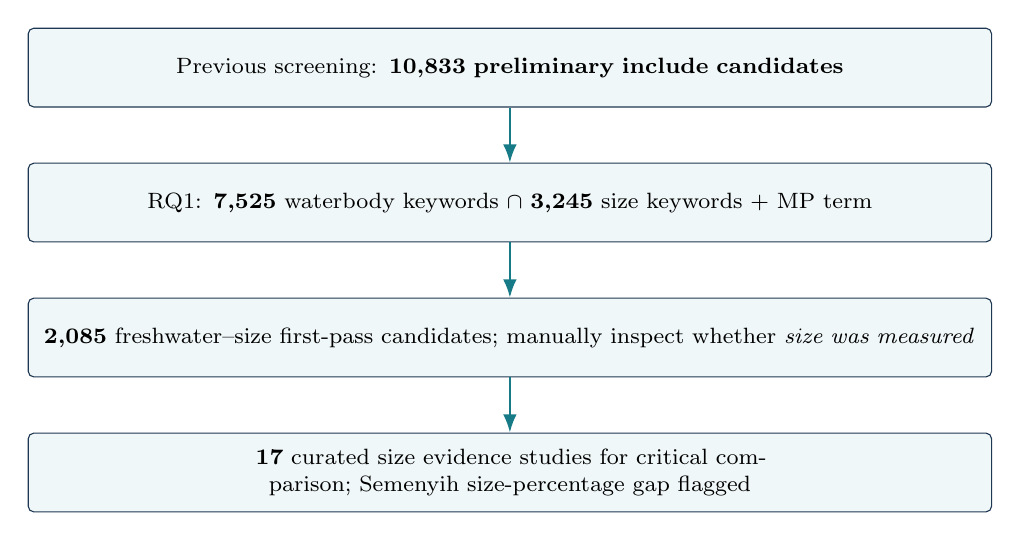
\begin{tikzpicture}[>=Latex, every node/.style={font=\footnotesize}, b/.style={draw=navy,rounded corners=2pt,fill=pale,minimum height=10mm,align=center,text width=12cm}, a/.style={->,thick,draw=teal}]
\node[b] (x) {Previous screening: \textbf{10,833 preliminary include candidates}};
\node[b,below=7mm of x] (y) {RQ1: \textbf{7,525} waterbody keywords $\cap$ \textbf{3,245} size keywords + MP term};
\node[b,below=7mm of y] (z) {\textbf{2,085} freshwater--size first-pass candidates; manually inspect whether \emph{size was measured}};
\node[b,below=7mm of z] (q) {\textbf{17} curated size evidence studies for critical comparison; Semenyih size-percentage gap flagged};
\draw[a] (x)--(y);\draw[a] (y)--(z);\draw[a] (z)--(q);
\end{tikzpicture}
\caption{Size-evidence filtering. The 17 examples are a transparent targeted sample, not the total number of eligible studies within 2,085 records.}\end{figure}

\subsection{How affiliation was filtered}
The \emph{Nottingham} query was run across corresponding/author-address and affiliation metadata, but \textbf{not} the author names alone. Campus confirmation required an explicit \texttt{UNIV NOTTINGHAM MALAYSIA} / \texttt{UNIVERSITY OF NOTTINGHAM MALAYSIA}, or an institutional Nottingham address locating the author in Semenyih; merely using a Nottingham email domain or a name such as ``University of Nottingham'' without Malaysia did not qualify. Each positive record is included in \texttt{data/UNM\_9\_Full\_Evidence.csv}, and each other Nottingham result in \texttt{data/Nottingham\_OtherCampuses\_24.csv}. This is \emph{all matches under the named database and rule}, not an exhaustive bibliography of the whole university beyond the database.

\subsection{Reproducibility: scripts and paper-level decisions}
This Overleaf package contains the actual Python screening code in the \texttt{scripts/} subfolder. The original implementation is preserved as \texttt{00\_original\_screening.py}; a revised executable version (\texttt{01\_screen\_candidates.py}) produces a flag and written selection reason for \emph{every one} of the 10,833 corpus records. The companion \texttt{curation\_size\_studies.csv} explicitly separates the \emph{human-reviewed} list of 17 size-evidence examples from the automatic first-pass screen. \texttt{03\_verify\_outputs.py} checks the counts, row identifiers and DOI uniqueness. An RStudio helper can identify and export a matching candidate data frame from the source \texttt{.RData}; that helper was supplied for local reproduction, not executed during this analysis.

\begin{table}[H]\centering\small
\caption{Screening code, input, outputs and permissible inference.}\label{tab:reproduce}
\begin{tabularx}{\linewidth}{@{}p{3.0cm}p{4.2cm}X@{}}\toprule
File or stage & Operation & Interpretation \\\midrule
Python first-pass script & Title/abstract keyword intersection for RQ1 & Generates 2,085 \emph{potentially relevant} freshwater-size records; not confirmed size reporting.\\
Human-curated DOI list & Manual DOI-based extraction of 17 studies & An explicitly curated example set, \emph{not} every eligible study among 2,085.\\
Affiliation query in Python & \texttt{C1}, \texttt{affiliations}, \texttt{AU\_UN}, \texttt{AU1\_UN}, \texttt{RP} & Nine strict UNM matches, 24 other/unclear Nottingham records; only within this exported corpus.\\
Row-level decision audit & Retains all original row IDs and positive/negative flags with reasons & Allows an investigator to review omissions and keyword false positives.\\
Verification script & Checks membership/count arithmetic & Verifies reproducibility of screening, \emph{not} validity of all study findings.\\
\bottomrule\end{tabularx}
\end{table}

The source \texttt{Include\_Candidates.csv} is not embedded in the Overleaf ZIP because it is a large, separately maintained project export. The README explains how to point the scripts to it on Windows. A newer source export with changed records or metadata must be handled as a new screening version, rather than silently mixing counts with this manuscript.

\section{RQ1: What microplastic sizes are common in rivers and ponds?}
\subsection{What comparison across studies can and cannot tell us}
A clear pattern in multiple \emph{measured} freshwater studies is that particles smaller than 0.5 or 1~mm are prominent, though the exact leading interval differs substantially by site and method \cite{Corpus15,Corpus05,Corpus17,Corpus11,Corpus04}. The opposite is possible: the Songhua River study reports roughly equal contributions from $\leq$1~mm and 1--5~mm classes \cite{Corpus10}. There is \textbf{no justified global modal size} to quote without harmonising lower detection limits, samplers, polymer verification, fibre measurement conventions, and particle-size definitions. A broader river meta-analysis cautions that sampling methods and missing hydrological context strongly affect apparent riverine MP concentrations \cite{Lofty2023}.

\subsection{Representative measured evidence from the screened papers}
\small
\begin{longtable}{@{}p{2.75cm}p{2.15cm}p{6.1cm}p{3.35cm}@{}}
\caption{Study-level size findings for freshwater surface water, with mixtures explicitly identified. Values are individual study observations, \emph{not pooled percentages}.}\label{tab:sizepapers}\\
\toprule Location/study & Matrix & Reported size evidence & Important interpretation\\\midrule\endfirsthead
\multicolumn{4}{l}{\footnotesize Table \thetable\ continued}\\\toprule Location/study & Matrix & Reported size evidence & Interpretation\\\midrule\endhead
Langat River, Malaysia \cite{Corpus04} & Surface water & $<300$: 6.64\%; 300--500: 14.19\%; 500--1000: 36.81\%; 1001--5000~$\mu$m: 42.36\% & Largest \emph{individual} bin is 1--5 mm; combined $<1$ mm is 57.64\%.\\
Selangor River Basin \cite{Corpus07} & Surface water & 600--1000~$\mu$m was the largest reported class, at 26.3\% & Regionally relevant; \emph{not} Semenyih.\\
Cherating River \cite{Corpus01} & Aquatic study & 0.5--1.0~mm reported prevalent & Malaysia study; full text needed for exact fraction.\\
Tropical urban ponds, India \cite{Corpus11} & Pond surface water & 500--1000~$\mu$m was the predominant size class & Based on bucket/tube-net samples.\\
Wei River, China \cite{Corpus15} & River water & $<0.5$ mm constituted 68.1\% & Small fraction dominant in this study.\\
Lhasa River, China \cite{Corpus05} & River surface water & 0--0.5 mm constituted 75.83\% & Abstract report of river-water class.\\
Yellow River, Lanzhou \cite{Corpus17} & River water & $<1$ mm constituted 83.67\% & Size and shape jointly discussed.\\
Vaal River, South Africa \cite{Corpus13} & River surface water & 0.06--4.95 mm detected; over 89\% under 2 mm & Broad range; not same bin system.\\
Vaal River, South Africa \cite{Corpus12} & Water and sediment & Over 80\% were smaller-than-2-mm fragments/fibres & Combined size-and-shape statement; matrix separation required.\\
Nhue--Day basin, Vietnam \cite{Corpus06} & River water & 0.5--2 mm: 71--100\% at reported stations & Station-dependent fraction.\\
Songhua River, China \cite{Corpus10} & River water & $\leq 1$ mm and 1--5 mm: approximately 50\% each & Counterexample to universal smaller-size dominance.\\
Songhua River, China \cite{Corpus09} & Surface water & $<0.5$ mm and 0.5--1 mm were main classes & No exact combined percentage in abstract.\\
Wei River Plain \cite{Corpus14} & Surface waters & $<0.5$ mm dominant & Exact share not in abstract.\\
Wei River, China \cite{Corpus16} & River water & $<500~\mu$m dominant & Consistent regional example.\\
Seasonal freshwater ponds \cite{Corpus02} & Pond surface water & $<1000~\mu$m commonly observed & Pond water; season and sampling matter.\\
Lake Gahai, China \cite{Corpus03} & Lake water & 20--50~$\mu$m: 64.42\% & Highlights micro-scale detections in sensitive methods.\\
Semenyih River \cite{Corpus08} & Water and bed & \textbf{No reliable size-class percentages in abstract} & Do not invent a local histogram.\\
\bottomrule
\end{longtable}\normalsize

\subsection{Semenyih River: the primary local finding}
Chen \emph{et al.} reported 160 samples from eight Semenyih River sites (replicates over three dates), with MPs detected in every sample. Mean river-water abundance was \textbf{3.12 $\pm$ 2.49 particles/L}; bed-surface abundance was \textbf{6027.39 $\pm$ 16,585.87 particles/m$^2$}. \textbf{Fibres dominated} the observed types; fragments were proportionally more important on the bed than in the water. Variability among replicates at a site was high, and water and riverbed hotspots did not coincide \cite{Corpus08}. This is valuable spatial and morphology evidence but \textbf{does not establish the predominant Semenyih MP diameter}.

\begin{figure}[H]\centering
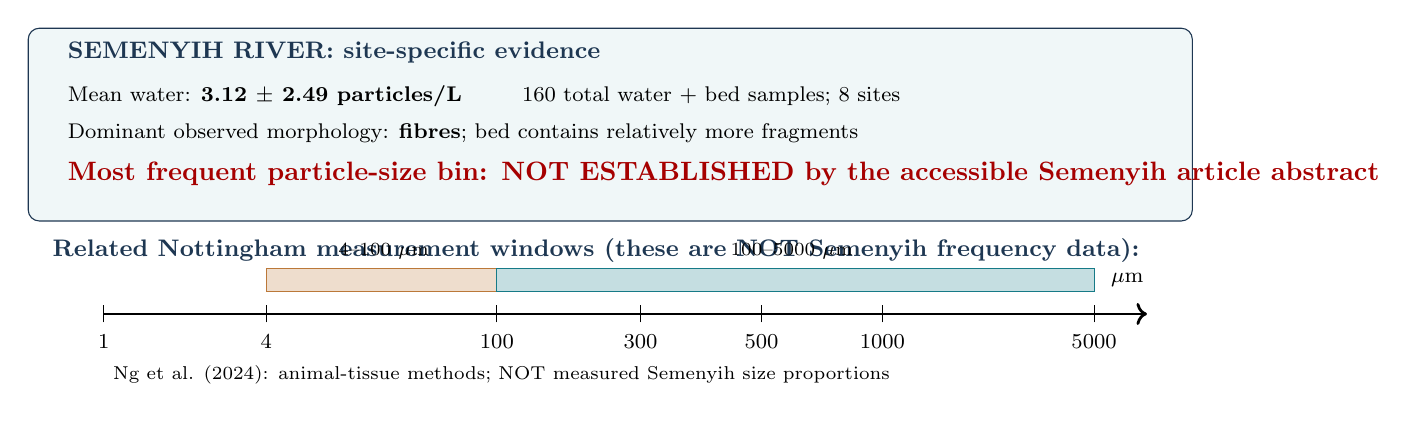
\begin{tikzpicture}[font=\footnotesize,scale=0.96,transform shape]
\draw[fill=pale,draw=navy,rounded corners] (0,1.5) rectangle (15.4,4.05);
\node[anchor=west,font=\bfseries\small,text=navy] at (.4,3.73) {SEMENYIH RIVER: site-specific evidence};
\node[anchor=west] at (.4,3.15) {Mean water: \textbf{3.12 $\pm$ 2.49 particles/L} $\qquad$ 160 total water + bed samples; 8 sites};
\node[anchor=west] at (.4,2.66) {Dominant observed morphology: \textbf{fibres}; bed contains relatively more fragments};
\node[anchor=west,text=red!65!black,font=\bfseries] at (.4,2.13) {Most frequent particle-size bin: NOT ESTABLISHED by the accessible Semenyih article abstract};
\node[anchor=west,font=\bfseries\small,text=navy] at (.2,1.11) {Related Nottingham measurement windows (these are NOT Semenyih frequency data):};
\draw[->,line width=1pt] (1,0.27)--(14.8,0.27);
\foreach \x/\t in {1/1,3.15/4,6.2/100,8.1/300,9.7/500,11.3/1000,14.1/5000}{\draw (\x,.16)--(\x,.39);\node[anchor=north] at (\x,.12) {\t};}
\node[anchor=west] at (14.2,.72) {$\mu$m};
\draw[fill=gold!25,draw=gold] (3.15,.57) rectangle (6.2,.87);
\draw[fill=teal!25,draw=teal] (6.2,.57) rectangle (14.1,.87);
\node[anchor=south,font=\scriptsize] at (4.7,.87) {4--100 $\mu$m};
\node[anchor=south,font=\scriptsize] at (10.1,.87) {100--5000 $\mu$m};
\node[anchor=west,font=\scriptsize] at (1,-.53) {Ng et al. (2024): animal-tissue methods; NOT measured Semenyih size proportions};
\end{tikzpicture}
\caption{Semenyih-focused evidence diagram. Top: actual local field findings \cite{Corpus08}. Bottom: the two \emph{method-capability} windows reported in related Nottingham research \cite{Corpus24}; bar length encodes a size range, \textbf{not} particle abundance. The actual modal size in Semenyih cannot be inferred.}\label{fig:semenyih}
\end{figure}

\subsection{Regional size-distribution comparator---Langat is not Semenyih}
\begin{figure}[H]\centering
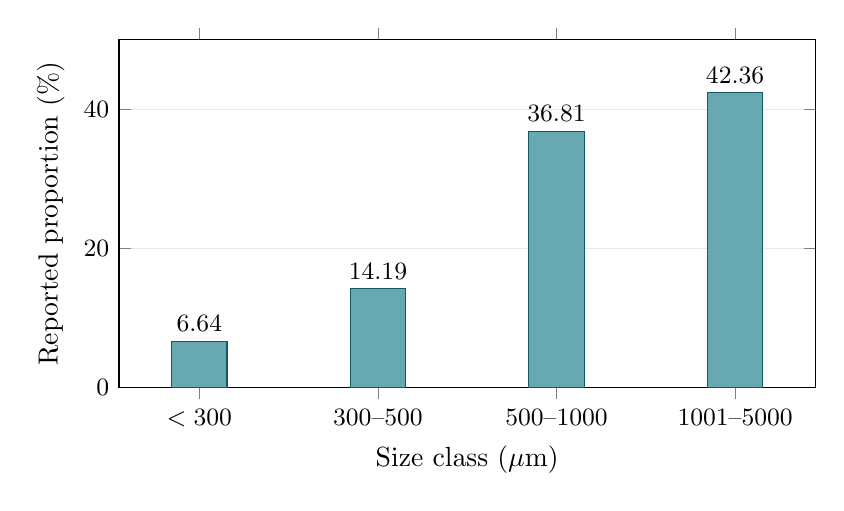
\begin{tikzpicture}
\begin{axis}[ybar,width=.86\linewidth,height=6.0cm,ymin=0,ymax=50,
 symbolic x coords={$<300$,$300$--$500$,$500$--$1000$,$1001$--$5000$},xtick=data,
 ylabel={Reported proportion (\%)},xlabel={Size class ($\mu$m)},
 nodes near coords, every node near coord/.append style={font=\small},
 ymajorgrids=true,grid style={gray!18},bar width=20pt,
 tick label style={font=\small},enlarge x limits=.15]
\addplot[draw=teal!75!black,fill=teal!65] coordinates {($<300$,6.64) ($300$--$500$,14.19) ($500$--$1000$,36.81) ($1001$--$5000$,42.36)};
\end{axis}
\end{tikzpicture}
\caption{\textbf{Langat River comparator ONLY}, reported by Mohd Ali \emph{et al.} \cite{Corpus04}. The proportion under 1,000~$\mu$m is 57.64\%. This is \emph{not} a Semenyih River plot or a pooled Malaysian distribution.}\label{fig:langat}
\end{figure}

\subsection{Implications for selecting a detection size cutoff}
For a practical Track A (live boat) or Track B (shoreline processing) device, an initial \textbf{100--1,000~$\mu$m or 100--5,000~$\mu$m} operational target can be considered for imaging-based counting, but would knowingly exclude smaller particles. These are proposed design ranges, not established Semenyih modal sizes. Fine fractions below 100~$\mu$m matter scientifically, as illustrated by the 20--50~$\mu$m lake measurements, but demand higher-resolution detection and more stringent contamination/verification controls \cite{Corpus03,Corpus24}. A robust output must state minimum measurable size, count-versus-mass units and handling losses. Filtration cutoffs and optical resolutions are separate quantities.

\section{RQ2: All explicit University of Nottingham Malaysia matches}
\subsection{Affiliation audit and completeness}
Nine records pass the strict campus affiliation rule. They cover \textbf{six primary/experimental contributions} and \textbf{three reviews or conceptual syntheses} after content appraisal. These are \emph{not} nine laboratory detection-accuracy experiments. A co-author's UNM address is sufficient for inclusion; it does \emph{not} prove that all experimental work was performed on campus or that every listed instrument is owned by UNM. Exact affiliations can be checked in the companion CSV.

\small
\begin{longtable}{@{}p{1.0cm}p{6.25cm}p{3.9cm}p{3.15cm}@{}}
\caption{Every paper with an explicit UNM affiliation in the 10,833 records, classified by its actual purpose.}\label{tab:unm}\\
\toprule Year & Paper & Technique / experimental role & Results / detection accuracy\\\midrule\endfirsthead
\multicolumn{4}{l}{\footnotesize Table \thetable\ continued}\\\toprule Year & Paper & Technique / role & Results / accuracy\\\midrule\endhead
2021 & Mofijur \emph{et al.}, sources, distribution and threats \cite{Corpus18} & Narrative review; no new UNM sample detection established & No empirical sensor-accuracy rate.\\
2021 & Chen \emph{et al.}, spatio-temporal Langat River \cite{Corpus20} & Repeated field sampling, preparation, visual microscopy; subset FTIR confirmation & 508 samples; mean 4.39 particles/L; \textbf{96\% visual identification agreement} in FTIR-checked $n=85$ subset.\\
2021 & Chen \emph{et al.}, Southeast Asian freshwater review \cite{Corpus21} & Literature review of levels, sources and impacts & No new experimental method accuracy.\\
2022 & Lee \emph{et al.}, U-Net counting \cite{Corpus23} & Microscope images + U-Net segmentation and post-processing & Human-level counting described; \emph{numerical accuracy not given in abstract}.\\
2022 & Chen \emph{et al.}, local riverborne sources \cite{Corpus25} & Water sampling, microplastic identification and source apportionment & Road culverts 42.20 $\pm$ 35.29 particles/L; reported WWTP removal efficiencies are \emph{not} accuracy.\\
2023 & Chen \emph{et al.}, Semenyih River water/bed \cite{Corpus08} & Replicated sampling, preparation and microscopy; bed density separation & 3.12 $\pm$ 2.49 particles/L water; no per-study detection-accuracy percentage given.\\
2023 & Hanun \emph{et al.}, weathered PET sorption \cite{Corpus22} & Controlled PET aging, SEM morphology, FTIR surface chemistry, BET, sorption & Sorption changes measured; \emph{not a river-water MP-counting accuracy study}.\\
2024 & Ng \emph{et al.}, fish and macroinvertebrates \cite{Corpus24} & Visual 0.1--5 mm and automated high-resolution 0.004--0.1 mm analysis & 95\% fish positive, 44\% macroinvertebrate positive (\emph{prevalence, not accuracy}).\\
2026 & Alowaisy \emph{et al.}, phytoplankton--plastic interactions \cite{Corpus19} & Review/conceptual synthesis of heavy metals and micro/nanoplastics & No new UNM detection-accuracy measurement.\\\bottomrule
\end{longtable}\normalsize

\subsection{UNM's documented laboratory workflow: what equipment is evidenced?}
\textbf{Evidence from Chen's doctoral thesis (not a new tenth paper in the 10,833 set).} The sampling and processing workflow is described in detail in Chapter 5 \cite{ChenThesis2023}:
\begin{enumerate}
 \item Collect river-water and bed samples and log replicated site/date information.
 \item Digest water-sample organic matter using \textbf{20 mL of 30\% hydrogen peroxide + 20 mL of 0.05 M iron(II) sulfate} (Fenton-type treatment), heated at approximately \textbf{60$^\circ$C for 30 minutes}.
 \item Filter water samples using \textbf{0.7-$\mu$m Whatman GF/F glass-microfibre filters}; oven-dry at approximately \textbf{60$^\circ$C for 24 h}.
 \item Visually examine and enumerate particles using a \textbf{Nikon SMZ1500 stereoscopic microscope}, approximately \textbf{4--180$\times$}; assign morphologies (fibres, fragments, films, beads).
 \item For sediment samples, additionally use a \textbf{53-$\mu$m sieve}, \textbf{saturated ZnCl$_2$ density separation}, and \textbf{Eppendorf 5810R centrifuge at 10,000 rpm for 10 minutes}, then examine recovered material.
\end{enumerate}
The cited research also reports \textbf{FTIR checks of a subset of visual identifications} \cite{Corpus20}. These instrument/model details are documented in the project-associated thesis and source paper, but a publication is not a campus asset inventory; verify current instrument access separately. Chemical workflows above require proper safety procedures and equipment and are described as reported methods, \emph{not recommended as an unsupervised shoreline protocol}.

\subsection{What does the reported ``96\% accuracy'' actually mean?}
The Langat River study states that FTIR checks of \textbf{85 visually classified particles} found \textbf{96\% correct visual identification} \cite{Corpus20}. This estimates performance of \emph{visually selected candidates in the checked subset}, conditional on sampling/selection. It is \textbf{not} a field-wide sensitivity, independent polymer-confirmation rate for every particle, filtration recovery, or true-negative specificity. It cannot be transferred automatically to a polarising-camera, EIS, or new AI device. The original U-Net study reports human-level image counting, but its searchable abstract does not provide a numeric percent to claim as a validation rate \cite{Corpus23}.

\begin{table}[H]\centering\small\caption{Do not mistake these published percentages for equivalent accuracy metrics.}\label{tab:metrics}
\begin{tabularx}{\linewidth}{@{}p{3.3cm}p{2.6cm}X@{}}\toprule
Source & Number & Meaning\\\midrule
Chen et al. (2021) \cite{Corpus20} & \textbf{96\%} ($n=85$) & Correct visual identification among a checked set using FTIR; \emph{not} sampling recovery.\\
Ng et al. (2024) \cite{Corpus24} & 95\% fish; 44\% macroinvertebrates & Organisms in which MPs were detected by the low-resolution method; \emph{not} detection sensitivity.\\
Chen et al. (2022) \cite{Corpus25} & 30.95--69.94\% & Wastewater-treatment-plant MP removal efficiencies; \emph{not} analytical accuracy.\\
Chen et al. (2023) \cite{Corpus08} & 160/160 positive samples & Prevalence across field samples; \emph{not} sensitivity, specificity or recovery.\\
Lee et al. (2022) \cite{Corpus23} & No abstract-level percentage & Qualitative ``human-level'' counting description; require full paper/test set for precision, recall and error.\\\bottomrule
\end{tabularx}\end{table}

\section{Critical synthesis and implications for the project}
\subsection{What was actually learned from the local research?}
\textbf{Semenyih water and bed need separate consideration:} neither the local samples nor the spatial maxima are interchangeable. Repeated stations and adequate sampled volumes are important for georeferenced maps \cite{Corpus08}. \textbf{Langat shows temporal change:} all 508 river-water samples contained MPs; abundance was 4.39 particles/L on average and much higher in some tributaries, with a positive relation to river discharge and sediment/turbidity indicators \cite{Corpus20}. \textbf{Sources matter:} road drainage was a larger local source than residential or industrial culverts in the source-apportionment study \cite{Corpus25}. \textbf{Size-resolution matters:} 2024 biological monitoring found much higher counts when the high-resolution method was used; this cannot be interpreted as a measured river-water size distribution \cite{Corpus24}. \textbf{Imaging is feasible but not chemically specific:} the UNM U-Net contribution accelerates counts on microscope images, whereas chemical confirmation is a separate test \cite{Corpus23,Corpus20}.

\subsection{Track A versus Track B for a 2D map}
\begin{table}[H]\centering\small\caption{Method implications based on the findings and the restriction on routine specialist laboratory access.}
\begin{tabularx}{\linewidth}{@{}p{2.9cm}XX@{}}\toprule
Issue & Track A: live measurement & Track B: collected sample, shore processing\\\midrule
Size threshold & Flow-cell path and optics impose minimum size; must state it & Filter/pore size and microscope resolution each need calibration\\
Concentration at 3.12 particles/L & Low counts require adequate observed water volume and longer averaging & Larger known-volume samples can be collected and analysed in batches\\
Small particles & Especially difficult at high flow in complex water & Portable enrichment/microscopy may help, but below 100~$\mu$m challenging\\
UNM comparison & U-Net concept potentially adaptable but does not solve polymer selectivity & Local microscopy/FTIR studies offer precedent for a controlled reference procedure\\
Evidence standard & Particle count/L + known sensor volume + false-positive testing & Particle count/L + recovered fraction + blanks; optional limited external polymer ID\\
Map output & Continuous or segmented estimates, with latency and QC labels & Discrete geotagged observations, followed by interpolation with held-out checks\\\bottomrule
\end{tabularx}\end{table}

\subsection{Recommended next evidence request}
To produce an \emph{actual Semenyih percentage-by-size histogram}, obtain the corresponding particle-level dataset or full size-class table (if collected) from Chen et al. (2023) or the authors' thesis attachments. The published source indicates that the corresponding-author dataset is available on reasonable request \cite{Corpus08}. Obtain the original measured particle dimensions, morphology, sample size, minimum measurable size, and polymer-confirmation status; re-bin only after obtaining them. Do not substitute Langat or other Malaysian river fractions. If the team generates new data, retain raw images, calibration scales, size-bin definitions, blanks, volume, sampling date, and GPS coordinates.

\section{Study limitations and evidence-status statement}
The 17 size papers are a reproducible \emph{curated example set} drawn from 2,085 preliminary text matches, \textbf{not exhaustive final full-text inclusion}. The nine UNM papers are exhaustive under the explicit affiliation rule \emph{within this specific 10,833-record corpus}. University-owned laboratory inventory, transfer of methods to a new sensor, unreported detection efficiencies, and original Semenyih size frequencies cannot be inferred from abstracts. Any claims taken from the source thesis or publisher full text are distinguished from the corpus-wide title/abstract screening. Direct comparisons among studies require harmonised sampling method, minimum size, sample matrix, counting units, polymer identification and quality assurance \cite{Lofty2023}.
\printbibliography[title={IEEE-style references with DOI links}]
\end{document}
